% the sample slide is created with 16:9 aspect ratio
\documentclass[aspectratio=169,xcolor=dvipsnames]{beamer}

\usepackage{datetime2}
\DTMsetdatestyle{iso}

%\usepackage{xcolor}
\usepackage{forest}
\usepackage{adjustbox}
\usepackage{hyperref}

\ExplSyntaxOn
\NewDocumentCommand{\printrange}{m m}
{
	\int_eval:n { 1+#1*#2 } - \int_eval:n { (1+#1)*#2 }
}
\ExplSyntaxOff

% remove the options if you do not want to have them
\usetheme[
	% background=images/background.jpg, % you can add your own background image
	logo=images/kitchensink.png,
	sidelogo=images/research-horizontal.png,
]{unsw}
% uncomment to show notes. Works very nicely with dspdfviewer. You get something similar to PPT's presenter view.
%\usepackage{pgfpages}
%\setbeameroption{show notes on second screen}

% information for the title page
%\author{Samuel Marks, PhD}
\title{kitchenSink.ai}
\def\myTitle{kitchenSink.ai}
\subtitle{The only way to claim SOTA is to benchmark against the rest}
\institute{}%https://kitchenSink.ai}

\date{}
%\date{ \today}

\begin{document}
% use plain option to remove the page number from the title slide
\begin{frame}[plain]
	\titlepage
\end{frame}

\begin{frame}{Introduction}
	\textbf{Fractionated ML}\\
	The ML field is moving too rapidly. There is little confidence to be found in SOTA claims (e.g., in medicine).
\end{frame}

\begin{frame}{Team}
	\framesubtitle{Samuel Marks}
	\begin{block}{Academic}
		PhD from University of Sydney. On 2nd PhD at UNSW. Researcher at HMS/MEEI.
	\end{block}

	\begin{exampleblock}{Commercial}
		Delivered many dozens of projects for dozens of companies over 10+ years.
	\end{exampleblock}

	\begin{alertblock}{Charitable}
		Working on facilitating mass screening programmes for blinding eye diseases.
	\end{alertblock}
\end{frame}

\begin{frame}
	\begin{forest} for tree={grow'=0,anchor=west,child anchor=west},
		[\textbf{ML framework degrees of freedom},for tree={fill=BlueViolet,text=white}
				%[ML,for tree={fill=BlueViolet,text=white}
						%[Framework,for tree={}
								[CNN,fill=Bittersweet]
								[RNN,fill=Bittersweet]
								[Transformers,fill=Bittersweet]
								[Gradient boosting,fill=Bittersweet]
								[\textellipsis{},fill=Bittersweet,for tree={fill=JungleGreen}
									[Optimiser
									[Learning rate,fill=Mulberry]
									[\(\alpha\),fill=Mulberry]
									[\textellipsis{},fill=Mulberry]]
									[\textellipsis{}]
									[Loss]]
								[Ensembles,fill=Bittersweet]
								[Multimodal,fill=Bittersweet]]%]%]
	\end{forest}
\end{frame}

\part[foo]{bar}

\begin{frame}{Multi-ML}
	NOTE: The landscape is changing. I am a top 10 contributor to Google's [TensorFlow] Keras. A month ago they released a cross-compatible version that makes interchangeable: PyTorch, JAX, and TensorFlow.
\end{frame}

\begin{frame}{Multi-ML}
	There are ~10 commonly used ML frameworks. Each have different ecosystems, and when a new research paper---or industry project---is released, they (usually) target just one framework.\vspace{1em}

	My new multi-ML framework is created by applying my \href{https://pypi.org/project/python-cdd}{\texttt{\textbf{cdd-python}}} compiler to 10 different popular ML frameworks (at the source-code level). This exposes CLIs, REST APIs, database tables and other useful layers.\vspace{1em}

	Now, given a problem (e.g., determine best dataset for my new optimiser, or determine best [AUCROC] model for my new dataset), the framework will optimise across a \textit{search space} traversing permutations of parameters (e.g., optimiser, loss function) and hyperparameters (e.g, \(\alpha\), \(\beta\), learning rate). Where \textit{search space} can include everything that the ML ecosystem has to offer.
\end{frame}

{
\usebackgroundtemplate{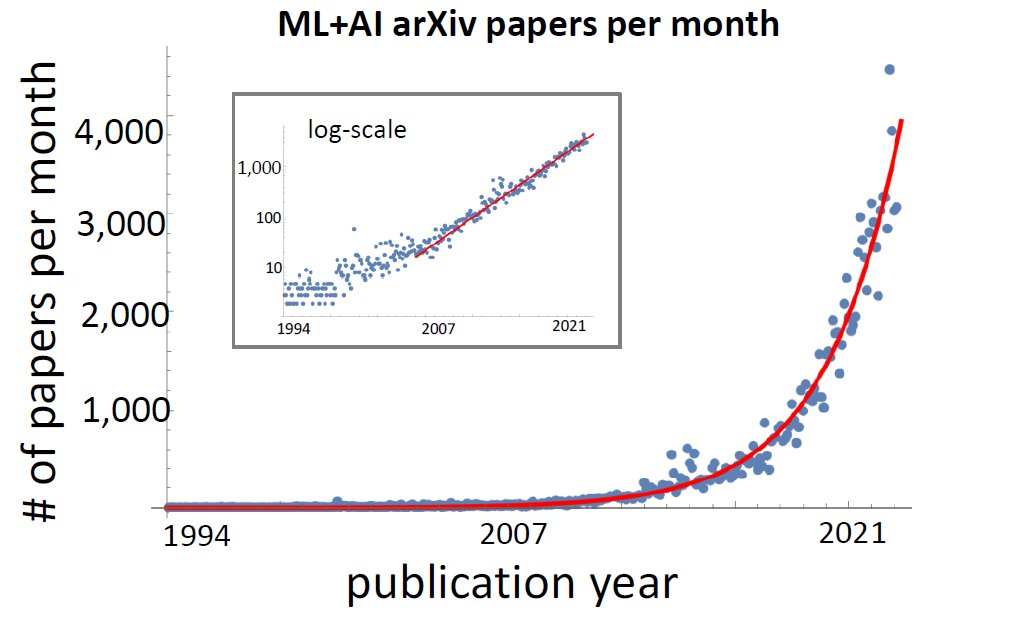
\includegraphics[width=\paperwidth]{images/number_of_AI_papers_on_arXiv_per_month.jpg}}
\begin{frame}[plain]
\end{frame}
}

\begin{frame}{Multi-ML - Future work \(\dfrac{I}{II}\)}
	Take arbitrary repos with Python packages or simple Notebooks \& automatically:

	\begin{enumerate}
		\item[0.] Find and clone candidate repositories (e.g., from the arXiv);
		\item Make OS independent;
		\item Remove absolute paths (e.g., to weight files);
		\item Format and autolint;
		\item Add type hints;
		\item Separate steps to be compatible with ensemble use-cases, e.g., move the model construction to its own function, and constants [like kernel sizes] to a consistent section;
		\item Send pull-request / merge-request to repository;
		\item If PR is accepted, add new model, optimizer, loss function, or other relevant `thing' to this multi-ML meta-framework's search-space;
		\item Publish (online) benchmarks of this new `thing' against similar `thing's on a variety of different datasets.
	\end{enumerate}
\end{frame}

\begin{frame}{Multi-ML - Future work \(\dfrac{II}{II}\)}
	\begin{enumerate}
		\item[0.] Automatically systematically review articles [with public datasets] coming through different research fields;
		\item run their claims against the entire search-space of this multi-ML meta-framework;
		\item (if improvement detected) write up a research paper with a new claim.
		\item (if improvement detected) Open-source the (new) result with clear replication steps.
	\end{enumerate}
	\vspace{2em}

	\begin{columns}
		\begin{column}[T]{0.4\textwidth}
			Add support for new ML frameworks.
		\end{column}
		\begin{column}[T]{0.4\textwidth}
			Analytics and dashboarding.
		\end{column}
	\end{columns}
\end{frame}

\end{document}
